\section{Orbiting}
\begin{frame}
	\frametitle{Orbiting}
		\textbf{Objective:} Algorithm to allow a planet to orbit around \textit{n} stars from any initial condition.
		\begin{itemize}
		\only<1->{
			\item \textbf{Stars:} Stationary bots around which planet rotates.
			\only<2->{
			\item \textbf{Planet:} Dynamic bots rotating around stars.
			}
		}
	\end{itemize}
\end{frame}

\begin{frame}
\frametitle{With single star}
\framesubtitle{Flowchart}
\begin{figure}[H]
	\centering
	\fbox{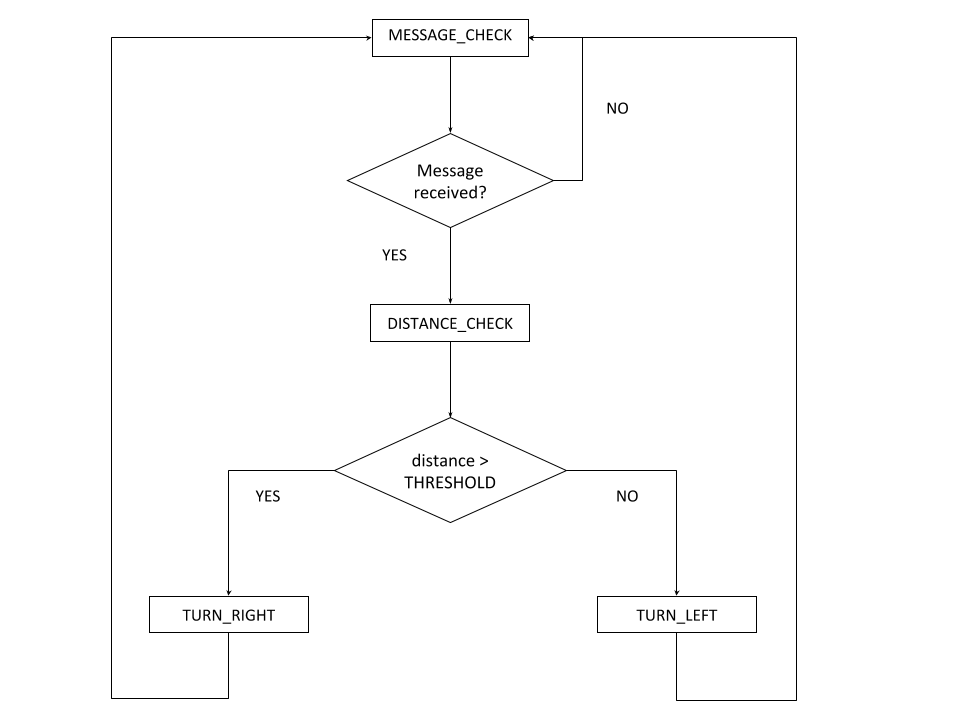
\includegraphics[width=3.6in]{images/flowchart-planet-star.png}}
	\caption{Flowchart for orbiting a Kilobot(Single star)}
	\label{fig:Flowchart_for_orbiting_a_Kilobot(Single_star)}
\end{figure}
\end{frame}

\begin{frame}
\frametitle{With single star}
\framesubtitle{Demonstration}
\begin{figure}[H]
	\centering
	\fbox{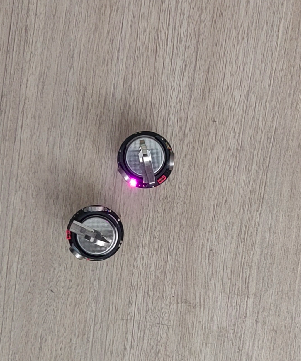
\includegraphics[width=2.0in]{images/planet-star-demo.png}}
	\caption{\href{https://drive.google.com/file/d/1fLfsFgo0ob07vIyrgzMQ1_RKYdbQMO9P/view}{Orbiting of Kilobot (Single Star)}}
	\label{fig:planet-star-demo}
\end{figure}
\end{frame}

\begin{frame}
\frametitle{With multiple stars}
\framesubtitle{Planet-Star Collision Demonstration}
\begin{figure}[H]
	\centering
	\fbox{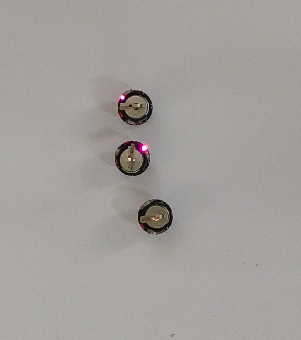
\includegraphics[width=2.0in]{images/planet-mstar-demo.png}}
	\caption{\href{https://drive.google.com/file/d/1OaW0ApBvJGrLmHM_Za6CWgqYbgkAapjx/view}{Planet colliding with one of the stars}}
	\label{fig:planet-star-collision}
\end{figure}
\end{frame}

\begin{frame}
\frametitle{With multiple stars}
\framesubtitle{Escaping the close region}
\textbf{Objective:} Designing a robust algorithm to reach the desired orbit distance without hitting the star.
\end{frame}

\begin{frame}
\frametitle{With multiple stars}
\framesubtitle{Flowchart}
\begin{figure}[H]
	\centering
	\fbox{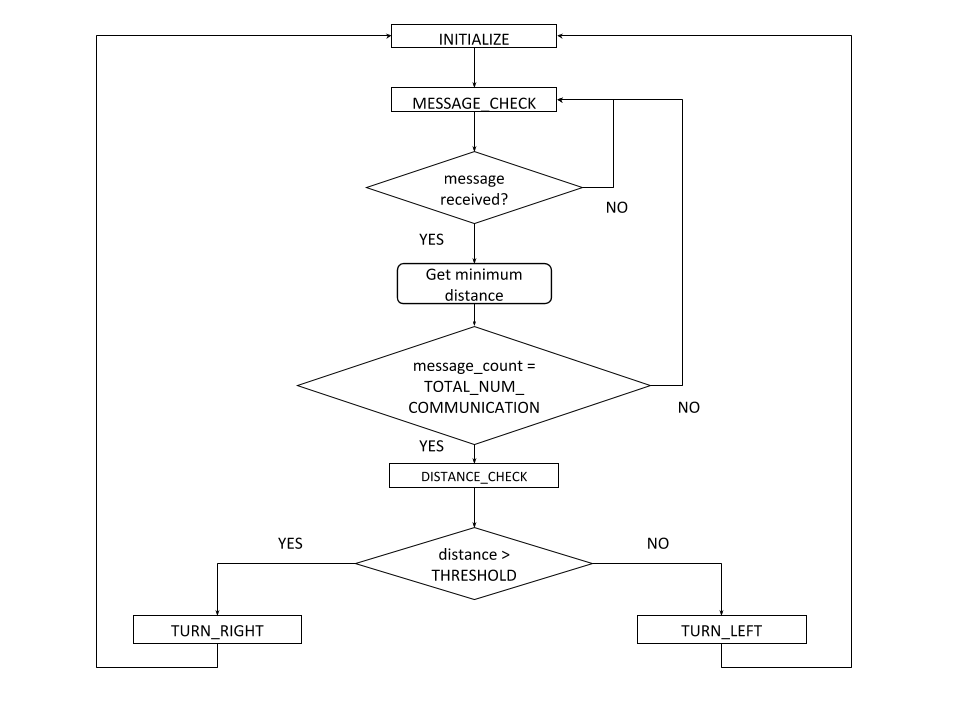
\includegraphics[width=3.5in]{images/flowchart-planet-mstar.png}}
	\caption{Flowchart for orbiting a Kilobot(Multiple star)}
	\label{fig:Flowchart_for_orbiting_a_Kilobot(Multiple_star)}
\end{figure}
\end{frame}

\begin{frame}
\frametitle{With multiple stars}
\framesubtitle{Demonstration}
\begin{columns}[b]
	\begin{column}{0.5\textwidth}
		\begin{figure}[H]
        	\centering
        	\fbox{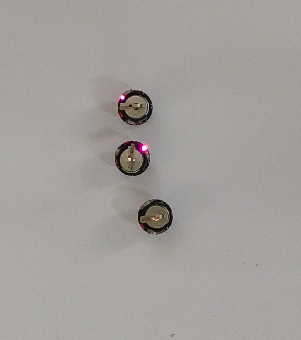
\includegraphics[width=1.3in]{images/planet-mstar-demo.png}}
        	\caption{\href{https://drive.google.com/file/d/1L9QUJOXNgUptjlVbOFi7709xdnPbLLnf/view}{Orbiting of Kilobot (Multiple Star, {\it MOTOR\_ON\_DURATION = 500}, {\it TOTAL\_NUM\_COMMUNICATION = 4})}}
        	\label{fig:planet-mstar-demo-1}
        \end{figure}
	\end{column}
	\begin{column}{0.5\textwidth}	
		\begin{figure}[H]
        	\centering
        	\fbox{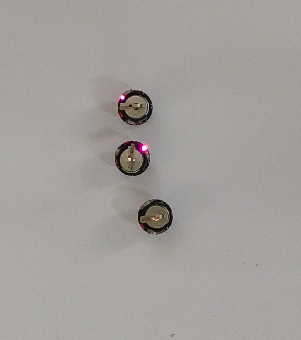
\includegraphics[width=1.3in]{images/planet-mstar-demo.png}}
        	\caption{\href{https://drive.google.com/file/d/1uEPULMZj-hb8SObypaLxKwzrtphcz_XN/view}{Orbiting of Kilobot (Multiple Star, {\it MOTOR\_ON\_DURATION = 800}, {\it TOTAL\_NUM\_COMMUNICATION = 3})}}
        	\label{fig:planet-mstar-demo-2}
        \end{figure}
	\end{column}
\end{columns}
\end{frame}